\documentclass{article}

\usepackage[main=english,vietnamese]{babel}
\usepackage[T1]{fontenc}
\usepackage[utf8]{inputenc}
\usepackage[sexy]{evan}
\usepackage{matchsticks}
\usepackage{wrapfig}
\usepackage{listings}

\newtheorem{hint}{Hint}

\title{Derivative}
\author{Nghia Doan}
\date{\today}

\begin{document}

\maketitle

\begin{definition*}[Injective function]
    An \textcolor{orange}{injective} function (\Cref{fig:injective}), 
    also known as \textbf{injection}, or \textbf{one-to-one function}, is a function
    that maps distinct elements of its domain to distinct elements of its codomain.
    \begin{center}
        If $f: X \mapsto Y$ is an injective if $\forall a,b \in X,\ f(a)=f(b) \Rightarrow a=b$.
    \end{center}
\end{definition*}

\begin{figure}[ht]
    \centering
	\begin{minipage}[t]{6.5cm}
        \centering
	    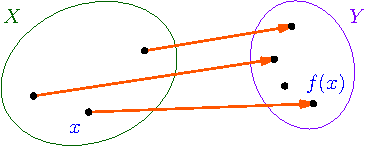
\includegraphics{./asy/pdf/injective.pdf}
        \caption{$f$ is injective}
        \label{fig:injective}
	\end{minipage}
\end{figure}

Every element of the codomain is the image of at most one element of its domain.
The term \textit{one-to-one function} must not be confused with \textit{one-to-one correspondence}
that refers to \textit{bijective} functions, which are functions such that each element in the codomain
is an image of exactly one element in the domain.

\newpage

\begin{problem*}[Problem 1]
    Let $f,g:\ \RR \rightarrow \RR$ be differentiable everywhere. Assume that $f$ is a one-to-one function.
    Show that 
    \[
        \left(f(g(x))\right)' = f'(g(x)) \cdot g'(x).
    \]
    without using any differentiation rules.
\end{problem*}

\begin{remark*}
    Assuming that $g$ is a one-to-one function.
\end{remark*}

\begin{remark*}
    There are a two notable facts:
    \begin{itemize}[topsep=0pt, partopsep=0pt, itemsep=0pt]
        \ii Since we cannot use any differentiation rules, it is likely that \textit{proof by definition} is the starting point.
        \ii The condition that $g$ is a one-to-one function is something that the chain rule does not assume.
    \end{itemize}

    Strategy: First, we look at the proof by definition \href{https://artofproblemsolving.com/ebooks/calculus-ebook/c3e1/label/5090}{how the chain rule is proved.}
    Second, we try to figure out why the additional condition might be useful.
    Finally, we will \textit{shorten} the official proof by using the condition.
\end{remark*}

\begin{soln}
    For any $x,$ note that
    \[
        \frac{f(g(x+h)) - f(g(x))}{h} = \left( \frac{f(g(x+h)) - f(g(x))}{g(x+h)-g(x)} \right) \left( \frac{g(x+h)-g(x)}{h}\right) \quad (*)
    \]

    Since $g$ is a one-to-one function, or $g(x+h) \ne g(x),$ none of the expressions on the left side has 0 as denominator,
    thus the limit of a product is a product of the limits,
    \[
        \lim_{h \rightarrow 0} \left( \frac{f(g(x+h)) - f(g(x))}{g(x+h)-g(x)} \right) \left( \frac{g(x+h)-g(x)}{h}\right)
        = \left( \lim_{h \rightarrow 0} \frac{f(g(x+h)) - f(g(x))}{g(x+h)-g(x)} \right) \cdot \left( \lim_{h \rightarrow 0} \frac{g(x+h)-g(x)}{h}  \right).
    \]
    
    Furthermore, $g$ is differentiable, thus continuous, so
    \[
        \lim_{h \rightarrow 0} g(x+h) = g(x) \Rightarrow \lim_{h \rightarrow 0} g(x+h) - g(x) = 0.
    \]

    Therefore
    \[
        \begin{aligned}
            &\lim_{h \rightarrow 0} \frac{f(g(x+h)) - f(g(x))}{g(x+h)-g(x)} = \lim_{h \rightarrow 0} \frac{f(g(x)+ (g(x+h) -g(x))) - f(g(x))}{g(x+h) -g(x)}\\
            &= \lim_{H_h = g(x+h)-g(x) \rightarrow 0} \frac{f(g(x)+ H_h)- f(g(x))}{H_h} = f'(g(x)).
        \end{aligned}
    \]

    Now,
    \[
        \left(f(g(x))\right)' =  \left( \lim_{h \rightarrow 0} \frac{f(g(x+h)) - f(g(x))}{g(x+h)-g(x)} \right) \cdot \left( \lim_{h \rightarrow 0} \frac{g(x+h)-g(x)}{h}  \right)
        = \boxed{f'(g(x)) \cdot  g'(x).}
    \]
\end{soln}

\newpage

\begin{problem*}[Problem 2a]
    Let $a \in \RR.$ Let $f$ be a function defined on $\RR.$
    Is each of the following claims true or false? Prove your answer.
    If it is true, prove it directly
    Hint: often times, the easiest way to prove something is false is by providing a counter example
    and proving that counter example satisfies the required conditions.

    (a) If the limit 
    \[
        \lim_{h \rightarrow 0} \frac{f(a+h) - 2f(a) + f(a-h)}{h^2}\ \text{exists,}
    \]
    then $f$ is twice differentiable at $x=a.$
\end{problem*}

\begin{remark*}
    Note that
    \[
        \frac{f(a+h) - 2f(a) + f(a-h)}{h^2} = \frac{1}{h} \left( \frac{f(a+h) - f(a)}{h} -  \frac{f(a) - f(a-h)}{h} \right) \quad (*)
    \]

    Thus the expression in (*) gives an \textit{impression} that if $f$ is (once) derivative then both left and right (first) derivatives would be the same,
    then the expression inside the parenthesis tends to $0,$ and the denominator outside of the parenthesis $h$ also tends to 0.
    However \textit{the rate of convergence might be different!}
    It means that if $f'(a+h)$ tends to $f'(a)$ in a different rate than $h$ tends to 0,
    in other words \textit{the second derivate of $f$ from the left and right sides of $a$ would have different values.}
    
    Therefore, we just need to find a function that
    \begin{itemize}[topsep=0pt, partopsep=0pt, itemsep=0pt]
        \ii Let pick $a=0$ for simplicity, $f$ is differentiable at $a,$ 
        \ii $f$ is twice differentiable at $a-$ and $a+$ but the values should be different;
        \ii $f$ should be selected so that the given equation stands.
    \end{itemize}
\end{remark*}

\begin{soln}
    We show a counter example,
    \[
        f(x) = 
        \begin{cases}
            x^2, &\text{if}\ x \ge 0\\
            0, &\text{if}\ x <0
        \end{cases}
    \]

    Then for $a=0,$
    \[
        \lim_{h \rightarrow 0} \frac{f(a+h) - 2f(a) + f(a-h)}{h^2} 
        = \lim_{h \rightarrow 0} \frac{h^2 - 2(0) + 0}{h^2} = 1.
    \]

    However $f$ is not twice differentiable, because
    \[
        \begin{aligned}
            &f'(x) = 
            \begin{cases}
                2x, &\text{if}\ x \ge 0\\
                0, &\text{if}\ x <0
            \end{cases}\\
            &f''(x) = 
            \begin{cases}
                2, &\text{if}\ x >0\\
                0, &\text{if}\ x <0\\
                \text{does not exist}, &\text{if}\ x=0
            \end{cases}\\
        \end{aligned}
    \]
\end{soln}

\begin{remark*}
    You can create a differentiable function that is not twice differentiable with almost any two differentiable functions,
    $f(x)$ and $g(x).$ If $f'(x) \ne g'(x)$ where you want to join them (at a, say),
    multiply $f'(x)$ by $g'(a)$ and $g'(x)$ by $f'(a),$ then add a constant to one of the functions to make them equal at $a.$
    Now the function is continuous and differentiable at $a,$ but not twice differentiable.
\end{remark*}

\newpage

\begin{problem*}[Problem 2b]
    (b) If there exists a function $m(x)$ such that
    \[
        f(x) - f(a) = m(x) (x-a),
    \]
    then $f$ is differentiable at $x=a.$
\end{problem*}

\begin{remark*}
    Note that
    \[
        f(x) - f(a) = m(x) (x-a) \Rightarrow m(x) = \frac{f(x) - f(a)}{x-a} \quad (*)
    \]

    Since there is no requirement for $m(x),$
    the limit $\lim_{x \rightarrow a} m(x)$ might not exist at all,
    thus the function $f$ would not be differentiable.

    We just need to chose an $f$ function that is not differentiable at $a$ by having $\lim_{x \rightarrow a} f(x) \ne f(a).$
\end{remark*}

\begin{soln}
    We show a counter example,
    \[
        f(x) = 
        \begin{cases}
            \frac{1}{x}, &\text{if}\ x \ne 0\\
            0, &\text{if}\ x = 0
        \end{cases}
    \]

    Let $m(x) = \frac{1}{x^2},$ for $a=0,$
    \[
        f(x) - f(a) = \frac{1}{x} - 0 = \frac{1}{x} = \frac{1}{x^2} (x - 0) = m(x) (x-a).
    \]

    $f$ is obviously not differentiable.
\end{soln}

\begin{remark*}
    The assumption for the existence of 
    \[
        \lim_{x \rightarrow a} \frac{f(x) - f(a)}{x-a}
    \]
    is very strong.
    It requires the existence of the limits on both sides of $a$ as well as the convergences result in the same value, which then should be the same as $f(a).$
\end{remark*}

\newpage

\begin{problem*}[Problem 3]
    Consider the function $f(x)$ given by the equation
    \[
        f(x) = 2023 + \cfrac{2023}{ 2022 + \cfrac{2022}{ 2021 + \cfrac{2021}{\ddots + \cfrac{2}{ 1+\cfrac{1}{x} } } } } 
    \]

    Find the equation of the line tangent to the graph of $f(x)$ at the point with $x-$coordinate 1.
    
    Hint: Construct a sequence of functions $f_1,$ $f_2,$ $f_3,$ $\ldots,$ $f_{2023}$ such that $f_{2023} = f(x).$
    Then use induction twice (to find $f'(1)$ and $f(1)$).
\end{problem*}

\begin{remark*}
    If 
    \[
        f_1(x) = 1 + \frac{1}{x},\ f_{n}(x) = n + \frac{n}{f_{n-1}(x)},\ \forall n \ge 2.
    \]
    
    then
    \[
        f_1(1) = 1 + \frac{1}{1} = 2,\ f_{2}(1) = 2 + \frac{2}{2} = 3,\ f_{3}(1) = 3 + \frac{3}{3} = 4.
    \]

    and
    \[
        f_{n}'(x) = -\frac{n}{(f_{n-1}(x))^2} \cdot f_{n-1}'(x) = (-1)^2\frac{n(n-1)}{(f_{n-1}(x) f_{n-2}(x))^2} \cdot f_{n-2}'(x)
    \]
\end{remark*}

\begin{soln}
    Let define the sequence of functions $f_1,$ $f_2,$ $f_3,$ $\ldots,$ $f_{2023},$ as follow:
    \[
        f_1(x) = 1 + \frac{1}{x},\ f_{n}(x) = n + \frac{n}{f_{n-1}(x)},\ \forall n \ge 2.
    \]

    It is easy to verify that $f_{2023}(x) = f(x).$

    First, we prove by induction that
    \begin{claim*}
        \[
            f_{n}(1) = n+1,\ \forall n\ge 1 \quad (*)
        \]
    \end{claim*}
    \begin{subproof}
        For the base case $n=1,$ 
        \[
            f_1(1) = 1 + \frac{1}{1} = 2.
        \]
    
        Let's assume that the hypothesis is true for $n,$ or
        \[
            f_{n}(1) = n+1.
        \]

        Then, 
        \[
            f_{n+1}'(1) = (n+1) + \frac{n+1}{f_{n}(1)} = (n+1) + \frac{n+1}{n+1} = n+2.
        \]

        Hence then hypothesis is true for all $n \ge 1.$
    \end{subproof}

\newpage

    Second, we prove by induction that
    \begin{claim*}
        \[
            f_{n}'(x) = \frac{(-1)^{n}n!}{(f_{n-1}(x) \cdot f_{n-2}(x) \cdots f_{1}(x) \cdot  x )^2} =\frac{(-1)^{n}n!}{\left(x \prod_{k=1}^{n-1} f_{k}(x) \right)^2},\ \forall n \ge 2 \quad (**)
        \]
    \end{claim*}
    \begin{subproof}
        Note that
        \[
            \begin{aligned}
                &f_{1}'(x) = \left( 1 + \frac{1}{x} \right) = -\frac{1}{x^2} = \frac{(-1)^1 \cdot 1!}{x^2}\\
                &f_{n}'(x) = -\frac{n}{(f_{n-1}(x))^2} \cdot f_{n-1}'(x),\ \forall n\ge 2
            \end{aligned}
        \]

        For the base case $n=2,$ 
        \[
            f_{2}'(x) = -\frac{2}{(f_{1}(x))^2} \cdot f_{1}'(x) = -\frac{2}{(f_{1}(x))^2} \cdot \frac{(-1)^1 \cdot 1!}{x^2} = \frac{(-1)^2 2!}{(xf_{1}(x))^2}.
        \]
    
        Let's assume that the hypothesis is true for $n,$ or
        \[
            f_{n}'(x) = \frac{(-1)^{n}n!}{(x \prod_{k=1}^{n-1} f_{k}(x))^2},\ \forall n \ge 2.
        \]

        Then, 
        \[
            f_{n+1}'(x) = -\frac{n+1}{(f_{n}(x))^2} \cdot f_{n}'(x) = -\frac{n+1}{(f_{n}(x))^2} \cdot f_{n}'(x) \cdot \frac{(-1)^{n}n!}{\left(x \prod_{k=1}^{n-1} f_{k}(x) \right)^2}
            = \frac{(-1)^{n+1}(n+1)!}{\left(x \prod_{k=1}^{n} f_{k}(x) \right)^2}.
        \]

        Hence then hypothesis is true for all $n \ge 2.$
    \end{subproof}

    Therefore, using both results (*) and (**),
    \[
        f'(1) = f_{2023}'(1) = \frac{(-1)^{2023}2023!}{\left(1 \cdot \prod_{k=1}^{2022} k+1\right) ^2} = \frac{(-1)^{2023}2023!}{(2023!)^2} = -\frac{1}{2023!}
    \]

    Thus the equation of the line tangent to the graph of $f(x)$ at the point with $x-$coordinate 1 is
    \[
        y = f'(1) (x-1) + f(1) = -\frac{1}{2023!} (x-1) + 2 = \boxed{-\frac{1}{2023!} x + \left(2 + \frac{1}{2023!}\right).}
    \]
\end{soln}

\newpage

\begin{problem*}[Problem 4ab]
    Let $f:\ \RR \rightarrow \RR$ be a function. We say that a non-empty set $U \subseteq \RR$ is \textbf{ajar} if
    \[
        \forall u \in U, \exists r > 0 \text{\ such that\ } (u-r, u+r) \subseteq U.
    \]

    (a) Show that $(0,2)$ is ajar.

    (b) Find a set that is not ajar. You don't need to prove it.
\end{problem*}

\begin{remark*}
    First, we prove it by using the definition, in other words, for an arbitrary $u \in U = (0,2),$ let's determine an $r$ such that
    \[
        (u-r, u+2) \subseteq U \Rightarrow 0 \le u - r < u + r \le 2 \Rightarrow r \le u, r \le 2 - u \Rightarrow r = \min(u, 2-u)
    \]

    For the second question, let's investigate the definition,
    \[
        \forall u \in U, \exists r > 0 \text{\ such that\ } (u-r, u+r) \subseteq U.
    \]
    
    $(u-r, u+r) \subseteq U$ means that some numbers smaller than $u$ must be inside $U.$
    It means that if $U$ contain a minimal or a maximal element, then it cannot be ajar,
    since no element smaller than the minimal (or larger than the maximal) would be in $U.$
    
    Let formally prove it. 
    Assume the contrary, let $m \in U$ be the minimal element of $U,$ then any number less than $m$ is not element of $U,$
    which mean that for any $r,$ the interval $(u-r, u+r)$ can not be contained entirely by $U,$ precisely
    \[
        \forall r > 0, \forall v:\ m-r < v < m, v \not \in U.
    \]

    Similarly, $U$ should not have a maximal element.

    It seems that the open boundary is a (necessary) condition for ajar intervals.
    Would an \textbf{ajar} set be a set of non-overlapping open intervals?
\end{remark*}

\begin{soln}
    Let an arbitrary $u \in U = (0,2),$ then $0< u < 2.$ Let $r = \min(u, 2-u),$ then $r > 0,$ and
    \[
        0 \le u-r \text{\ and\ } u+r \le 2 \Rightarrow 0 \le u - r < u + r \le 2 \Rightarrow (u-r, u+2) \subseteq (0,2) = U.
    \]

    Therefore $(0,2)$ is ajar.

    For the second question, let $U = [0, 2],$ then for $u=0 \in U,$ 
    \[
        \forall r > 0 \Rightarrow u-r = -r < 0 \Rightarrow (u-r, u+r) = (-r, r) \not \subseteq [0,2] = U.
    \]
\end{soln}

\newpage

\begin{problem*}[Problem 4c]
    In the following parts, we will use the two definitions:
    
    For $A \subseteq \RR,$ we define $f(A)\ :=\ \{ f(a):\ a \in A\}.$
    
    For $B \subseteq \RR,$ we define $f^{-1}(B)\ :=\ \{ x \in \RR:\ f(x) \in B\}.$

    Note that $f(A)$ and $f^{-1}(B)$ are both sets.

    (c) Show that $\forall a \in \RR, \forall \epsilon > 0, \exists \delta > 0,$ such that
    \[
        f((a-\delta, a+\delta)) \subseteq (f(a) - \epsilon, f(a) + \epsilon) \quad (*)
    \]
    is equivalent to the definition of $f$ is continuous everywhere.
\end{problem*}

\begin{soln}
    Let rewrite the statement (*):
    \[
        \forall a \in \RR, \forall \epsilon > 0, \exists \delta > 0, \forall x \in (a-\delta, a+\delta):\ f(a) - \epsilon \le f(x) \le f(a) + \epsilon \quad(S1)
    \]

    On the other hand, we say that $f$ is continuous at a point $a$ in the domain of $f,$ if 
    \[
        \lim_{x \rightarrow a} f(x) = f(a) \Leftrightarrow 
        \forall \epsilon > 0,\ \exists \delta > 0,\ \forall x:\  0 < |x-a| < \delta \Rightarrow |f(x)-f(a)| < \epsilon \quad (S2)
    \]
    
    We prove the two statements are equivalent in two directions.

    \begin{claim*}
        (S1) $\Rightarrow$ (S2).
    \end{claim*}
    \begin{subproof}
        Rewriting (S1) using the symbol $\gamma,$ instead of $\epsilon,$ and $\omega$ instead of $\delta$: for an arbitrary $a \in \RR,$
        \[
            \forall \gamma > 0, \exists \omega > 0, \forall x \in (a-\omega, a+\omega):\ f(a) - \gamma \le f(x) \le f(a) + \gamma \quad (1)
        \]
    
        So, for an arbitrary $a \in \RR,$ we need to use (1) to find a value for $\delta$ base on an arbitrary $\epsilon$ so that S(2) stands.
        
        Now, for a given arbitrary $\epsilon,$ by choosing $\gamma = \half \epsilon,$ we have, for $\gamma = \half \epsilon,$
        \[
            \begin{aligned}
                &\exists \omega > 0, \forall x \in (a-\omega, a+\omega):\ f(a) - \epsilon < f(a) - \half\epsilon \le f(x) \le f(a) + \half\epsilon < f(a) + \epsilon\\
                \Rightarrow\ &\exists \omega > 0, \forall x:\  0 < |x-a| < \omega \Rightarrow |f(x) - f(a)| < \epsilon < f(a) \quad (2)
            \end{aligned}
        \]

        Hence, by choosing  $\gamma = \half \epsilon,$ $\delta = \omega,$ and applied (1) as shown above, we received (2), which is
        \[
            \forall \epsilon, \exists \delta > 0,\ \forall x:  0 < |x-a| < \delta \Rightarrow |f(x)-f(a)| < \epsilon
        \]

        This is exactly S2.
    \end{subproof}

    \begin{claim*}
        (S2) $\Rightarrow$ (S1).
    \end{claim*}
    \begin{subproof}
        
        Rewriting (S2) using the symbol $\gamma,$ instead of $\epsilon,$ and $\omega$ instead of $\delta$: for an arbitrary $a \in \RR,$
        \[
            \forall \gamma > 0,\ \exists \omega > 0,\ \forall x:\  0 < |x-a| < \omega \Rightarrow |f(x)-f(a)| < \gamma \quad (3)
        \]
    
        So, for an arbitrary $a \in \RR,$ we need to use (1) to find a value for $\delta$ base on an arbitrary $\epsilon$ so that S(1) stands.
        
        Hence, by choosing  $\gamma = \epsilon,$ $\delta = \omega,$ and applied (3), we received
        \[
            \forall \epsilon, \exists \delta > 0,\ \forall x \in (a-\delta, a+\delta): f(a) - \epsilon \le f(x) \le f(a) + \epsilon \quad (4)
        \]

        Note that the inequalities in (4) are weakened from (3), which is perfectly correct to be done so. This is exactly S1.
    \end{subproof}
\end{soln}

\newpage

\begin{problem*}[Problem 4d]
    (d) Assume  that $f$ is continuous everywhere. Show that for any non-empty subset $U \subseteq \RR,$ 
    if $U$ is ajar, then $f^{-1}(U)$ is ajar. 

    Hint: To prove this, you need to prove and use these facts:
    \begin{enumerate}[topsep=0pt, partopsep=0pt, itemsep=0pt]
        \ii for all non-empty $A \subseteq \RR,$ $A \subseteq f^{-1}(f(A)).$ This should be one-line proof. 
        \ii $f^{-1}(B_1) \subseteq f^{-1} (B_2)$ if non-empty sets $B_1, B_2$ satisfies $B_1 \subseteq B_2 \subseteq \RR.$ This should be very short; and
        \ii the result from part (c)
    \end{enumerate}
\end{problem*}

\begin{soln}
    We prove the two facts. First, for the inverse image

    \begin{claim*}
        For all non-empty $A \subseteq \RR,$ $A \subseteq f^{-1}(f(A)) \quad (*)$  
    \end{claim*}
    \begin{subproof}
        By definition,
        \[
            x \in A \Rightarrow f(x) \in f(A) \Rightarrow x \in f^{-1}(f(A)) = \{ x \in \RR: f(x) \in f(A) \}
            \Rightarrow A \subseteq f^{-1}(f(A)).
        \]
    \end{subproof}

    Second, for the subsets
    \begin{claim*}
        If non-empty sets $B_1, B_2$ satisfies $B_1 \subseteq B_2 \subseteq \RR,$ then $f^{-1}(B_1) \subseteq f^{-1} (B_2) \quad (**)$ 
    \end{claim*}
    \begin{subproof}
        By definition, for non-empty sets $B_1, B_2$ satisfies $B_1 \subseteq B_2 \subseteq \RR,$
        \[
            \begin{aligned}
                &\forall e \in f^{-1}(B_1) \Rightarrow e \{ x \in \RR: f(x) \in B_1 \} \Rightarrow f(e) \in B_1 \subseteq B_2 \Rightarrow e \in f^{-1}(B_2)\\
                &\Rightarrow f^{-1}(B_1) \subseteq f^{-1} (B_2)
            \end{aligned}
        \]
    \end{subproof}

    Now, $f$ is continuous, by part (c), for an arbitrary $a \in \RR,$
    \[
        \forall \epsilon > 0, \exists \delta > 0:\ f((a-\delta, a+\delta)) \subseteq (f(a) - \epsilon, f(a) + \epsilon) \quad (1)
    \]

    $U$ is ajar, by definition,
    \[
        \forall f(a) \in U, \exists \epsilon > 0:\ (f(a)-\epsilon, f(a)+\epsilon) \subseteq U \quad (2)
    \]

    Apply (**) on (1), then (2),
    \[
        f^{-1}(f((a-\delta, a+\delta))) \subseteq f^{-1}((f(a) - \epsilon, f(a) + \epsilon)) \subseteq f^{-1}(U).
    \]

    By (*)
    \[
        (a-\delta, a+\delta) \subseteq f^{-1}(f((a-\delta, a+\delta))) \quad (3)
    \]

    This means $f^{-1}(U)$ is ajar, by (3):
    \[
        \forall a \in f^{-1}(U), \exists \delta > 0: (a-\delta, a+\delta) \subseteq f^{-1}(U).
    \]
\end{soln}

\newpage

\begin{problem*}[Problem 4e]
    (e) Assume that for any non-empty subset $U \subseteq \RR,$ if $U$ is ajar, then $f^{-1}(U)$ is ajar.
    Prove that $f$ is continuous everywhere. 

    Hint: Let $a\in \RR$ and $\epsilon >0,$ and consider the ajar set $(f(a) - \epsilon, f(a) + \epsilon)$ 
    (you might assume this set is ajar without proof.) You may also prove and use these facts.
    \begin{enumerate}[topsep=0pt, partopsep=0pt, itemsep=0pt]
        \ii for all non-empty $B \subseteq \RR,$ $f(f^{-1}(B)) \subseteq B.$
        \ii $f(A_1) \subseteq f(A_2)$ if non-empty sets $A_1, A_2$ satisfies $A_1 \subseteq A_2 \subseteq \RR.$ Both proofs should be very short; and
        \ii the result from part (c)
    \end{enumerate}
\end{problem*}

\begin{soln}
    We prove the two facts. First, for the inverse image

    \begin{claim*}
        For all non-empty $B \subseteq \RR,$ $f(f^{_1}(B)) \subseteq B \quad (*)$  
    \end{claim*}
    \begin{subproof}
        By definition, $f(f^{-1}(B)) = \{ f(a): a \in f^{-1}(B) \},$ so
        \[
            y \in f(f^{-1}(B)) \Rightarrow \exists x \in f^{-1}(B): y = f(x) \Rightarrow \exists x\in \RR, y = f(x) \in B
            \Rightarrow f(f^{_1}(B)) \subseteq B.
        \]
    \end{subproof}

    Second, for the subsets
    \begin{claim*}
        If non-empty sets $A_1, A_2$ satisfies $A_1 \subseteq A_2 \subseteq \RR:\ f(A_1) \subseteq f(A_2) \quad (**)$ 
    \end{claim*}
    \begin{subproof}
        By definition, for non-empty sets $A_1, A_2$ satisfies $A_1 \subseteq A_2 \subseteq \RR,$
        \[
            \begin{aligned}
                y \in f(A_1) = \{ f(a): a \in A_1 \} \Rightarrow \exists a \in A_1, y = f(a) \Rightarrow a \in A_2, y = f(a) \Rightarrow y \in f(A_2)
                \Rightarrow f(A_1) \subseteq f(A_2).
            \end{aligned}
        \]
    \end{subproof}

    Let $a\in \RR$ and $\epsilon >0,$ and consider the ajar set $U = (f(a) - \epsilon, f(a) + \epsilon).$

    $f^{-1}(U)$ is ajar,:
    \[
        \forall a \in f^{-1}(U), \exists \delta > 0: (a-\delta, a+\delta) \subseteq f^{-1}(U) \quad (1)
    \]

    Apply (**) on (1),
    \[
        f((a-\delta, a+\delta)) \subseteq f(f^{-1}(U)) \quad(2)
    \]

    By (*) on (1),
    \[
        f((a-\delta, a+\delta)) \subseteq f(f^{-1}(U)) \subseteq U = (f(a) - \epsilon, f(a) + \epsilon)
    \]

    This means, for an arbitrary $a \in \RR,$
    \[
        \forall \epsilon > 0, \exists \delta > 0:\ f((a-\delta, a+\delta)) \subseteq (f(a) - \epsilon, f(a) + \epsilon)
    \]

    By part (c), $f$ is continuous.
\end{soln}

\end{document}